\documentclass{scrreprt}
\usepackage[polish]{babel}
\usepackage[utf8]{inputenc}
\usepackage{listings}
\usepackage{graphicx}
\usepackage{aeguill}
\usepackage[bookmarks=true]{hyperref}
\hypersetup{
    bookmarks=false,    % show bookmarks bar?
    pdftitle={AGHydra - aimo},    % title
    pdfauthor={Yiannis Lazarides},                     % author
    pdfsubject={TeX and LaTeX},                        % subject of the document
    pdfkeywords={TeX, LaTeX, graphics, images}, % list of keywords
    colorlinks=true,       % false: boxed links; true: colored links
    linkcolor=blue,       % color of internal links
    citecolor=black,       % color of links to bibliography
    filecolor=black,        % color of file links
    urlcolor=purple,        % color of external links
}%
\def\myversion{1.0 }
\title{%
\flushright
\rule{16cm}{5pt}\vskip1cm
\Huge{Analiza\\ i Modelowanie Oprogramowania \\ - projekt}\\
\vspace{2cm}
dla\\
\vspace{2cm}
AGHydra System\\
\vspace{2cm}
Przygotowane przez:\\
Bartosz Śliwa\\
Michał Dziedzic\\
Daniel Poznański\\
\vfill
\rule{16cm}{5pt}
}
\date{}
\usepackage{hyperref}
\begin{document}
\maketitle
\tableofcontents
\chapter{Ogólny opis systemu}

\chapter{Analiza dziedziny}

\section{Słownik pojęć}
\begin{table}[ht]
	\centering
	\begin{tabular}{p{4cm}p{8cm}}
		\textbf{NAZWA}                     & \textbf{OPIS}                                                                                                       \\ \hline
		\multicolumn{1}{l|}{Firma}         & Określenie firm działających w branży IT, oferujących stanowiska stażowe lub normalne oferty pracy dla programistów \\ \hline
		\multicolumn{1}{l|}{System, Hydra} & całość rozwiązania składająca się z aplikacji frontowej i backendu                                                  \\ \hline
		\multicolumn{1}{l|}{UF}            & Uprawnienie funkcjonalne, wymagane do wykonania określonych akcji, przypisane do użytkownika                        \\ \hline
		\multicolumn{1}{l|}{Moduł}         & Wydzielona jako moduł Maven cześć aplikacji backendowej implementująca funkcjonalności w zakreślonym obszarze       \\ \hline
		\multicolumn{1}{l|}{Wiki}          & Moduł agregujący informacje na temat procesów rekrutacyjnych w firmach                                              \\ \hline
		\multicolumn{1}{l|}{Job}           & Moduł agregujący oferty pracy w firmach                                                                             \\ \hline
		\multicolumn{1}{l|}{Referral}      & Moduł umożliwiający tworzenie wewnętrznej rekrutacji do polecenia na dane stanowisko                                \\ \hline
		\multicolumn{1}{l|}{RA}            & Referral Announcement - ogłoszenie w dziale referral                                                                \\ \hline
	\end{tabular}
\end{table}

\section{Diagram obiektów biznesowych}
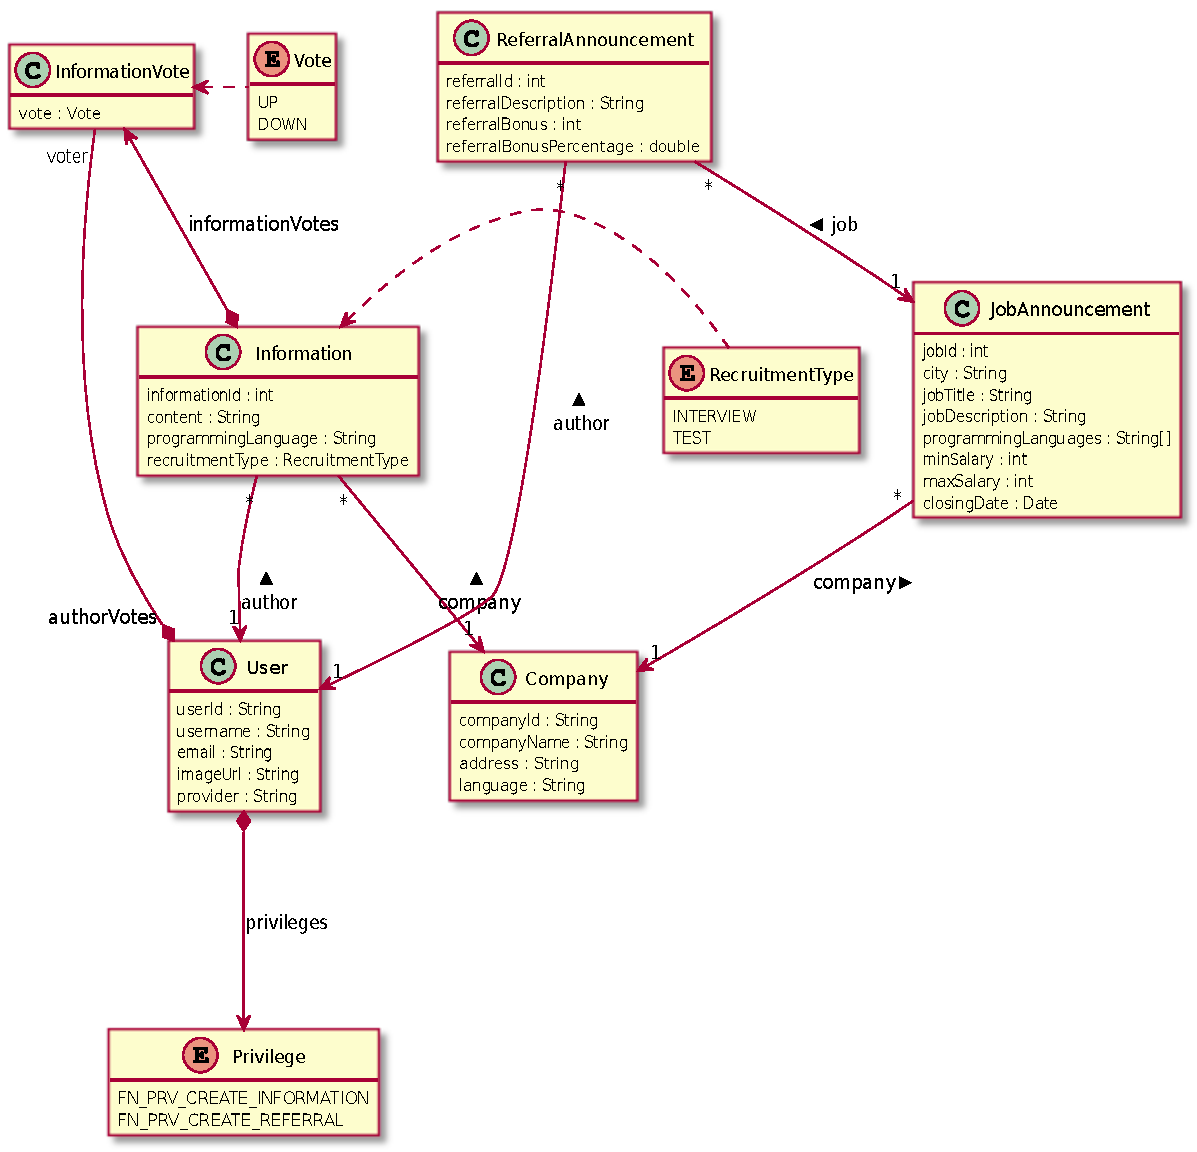
\includegraphics[width=\textwidth, keepaspectratio]{graphics/hydra_business_class_diagram.pdf}

\section{Opis obiektów biznesowych?}
//TODO: Danon

\section{Diagramy stanów}
//TODO: Danon

\chapter{SRS - Specyfikacja wymagań}
\section{Diagram przypadków użycia - Wiki}
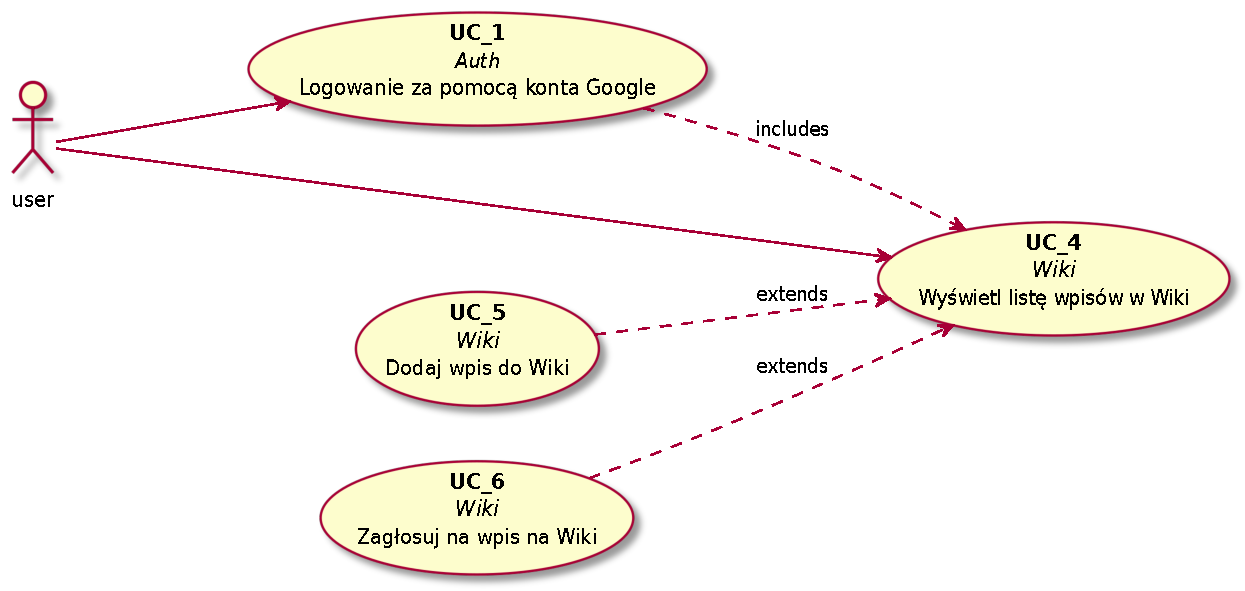
\includegraphics[width=\textwidth, keepaspectratio]{graphics/wiki_use_case_diagram.pdf}

\section{Diagram przypadków użycia - Job, Referral}
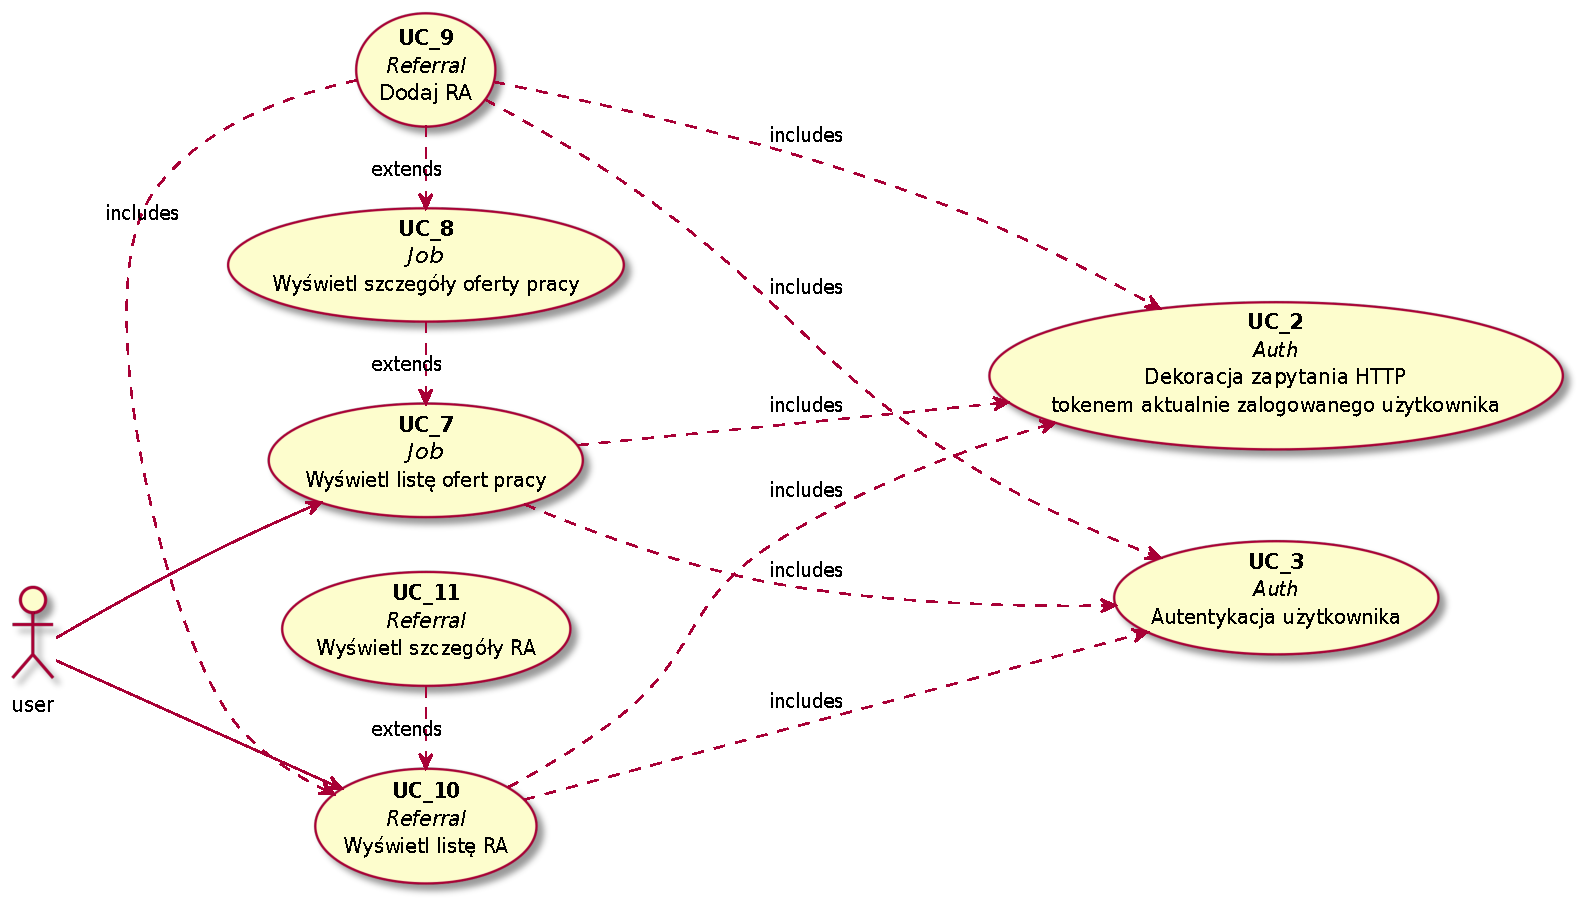
\includegraphics[width=\textwidth, keepaspectratio]{graphics/job_referral_use_case_diagram.pdf}

\section{Przypadki użycia powiązane z zabezpieczeniem dostępu}
\subsection{UC\_1 Logowanie za pomocą konta Google}
\subsection{UC\_2 Dekoracja zapytania HTTP tokenem aktualnie zalogowanego użytkownika}
\subsection{UC\_3 Autentykacja użytkownika}

\section{Przypadki użycia powiązane z Wiki}
\subsection{UC\_4 Wyświetl listę wpisów w Wiki}
\subsection{UC\_5 Dodaj wpis do Wiki}
\subsection{UC\_6 Zagłosuj na wpis na Wiki}

\section{Przypadki użycia powiązane z Job, Referral}
\subsection{UC\_7 Wyświetl listę ofert pracy}
\subsection{UC\_8 Wyświetl szczegóły oferty pracy}
\subsection{UC\_9 Dodaj RA}
\subsection{UC\_10 Wyświetl listę RA}
\subsection{UC\_11 Wyświetl szczegóły RA}


\chapter{Architektura systemu}

\section{Diagram komponentów}
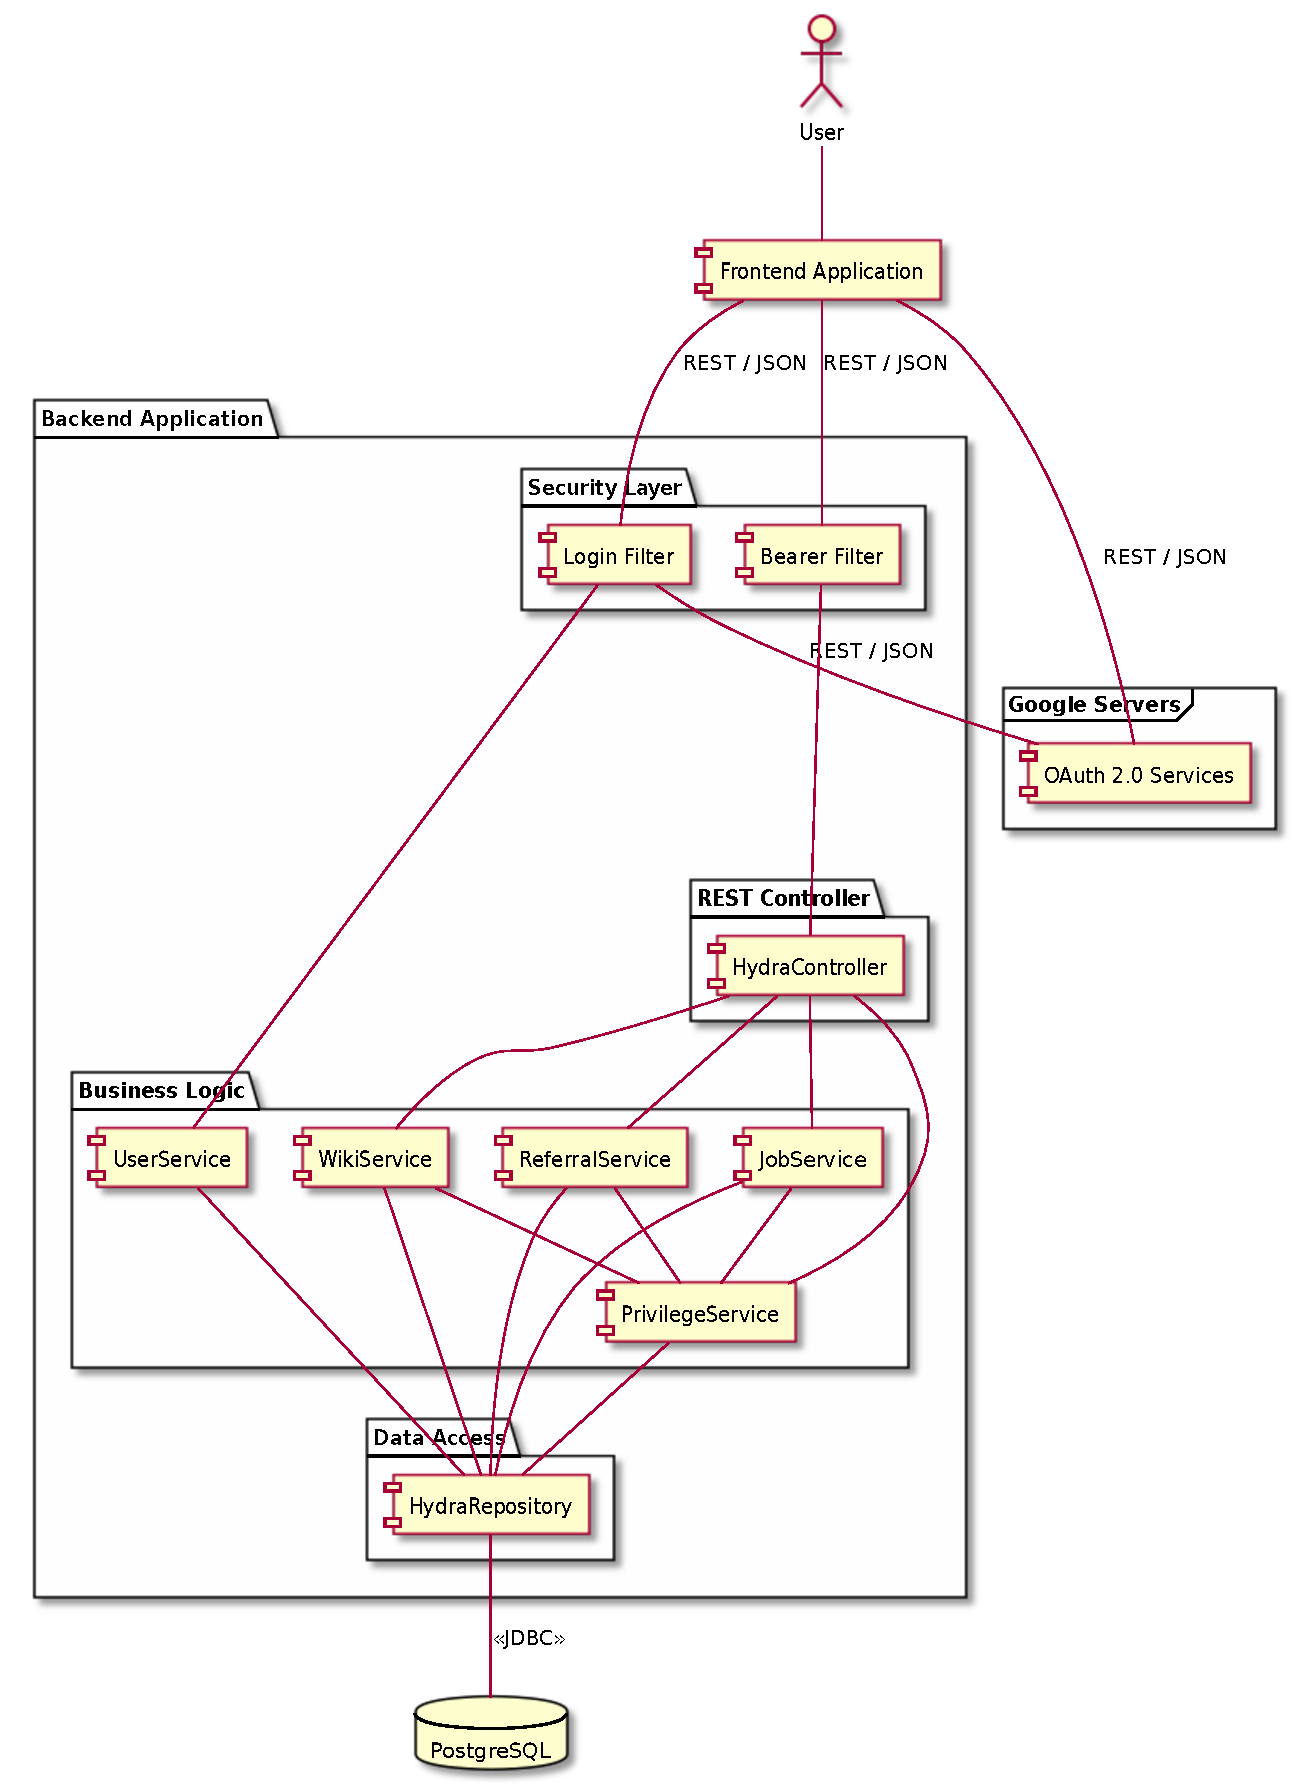
\includegraphics[width=\textwidth, keepaspectratio]{graphics/hydra_component_diagram.pdf}

\section{Opis warstw}
\subsection{Frontend Application}
Klient na platformy mobilne zrealizowany w języku \textbf{JavaScript} z wykorzystaniem frameworku \textbf{React Native}.
Pisany w ten sposób kod jest renderowany do natywnych implementacji Android \textit{(Java)} i iOS \textit{(Swift)}.

\subsection{Backend Application}
Serwer zrealizowany w technologii \textbf{Java} z wykorzystaniem biblioteki \textbf{Spring}

\subsubsection{Security Layer}
Warstwa odpowiada za zabezpieczenie dostępu do dalszych zasobów. 
Waliduje nadchodzące requesty na podstawie bearer tokena zawartego w ich nagłówkach.
Wychodząca odpowiedź serwera jest wzbogacana o odświeżony token i idektyfikator użytkownika.\\
Jedynym wyjątkiem w tym zabezpieczeniu jest próba logowania.

\subsubsection{REST Controller}
Komponenty te mapują zapytania do wywołań odpowiednich metod warstwy logiki biznesowej. 
Dodatkowo, nadchodzące requesty poddawane są walidacji pod kątem formatu zawartych danych.

\subsubsection{Business Logic}
Warstwa enkapsulująca logikę biznesową.

\subsubsection{Data Access}
Upraszcza innym komponentom integrację z informacjami przechowywanymi w bazie danych. 


\chapter{Projekt oprogramowania}

\subsection{Diagram klas}

\section{UC\_1 Logowanie za pomocą konta Google}
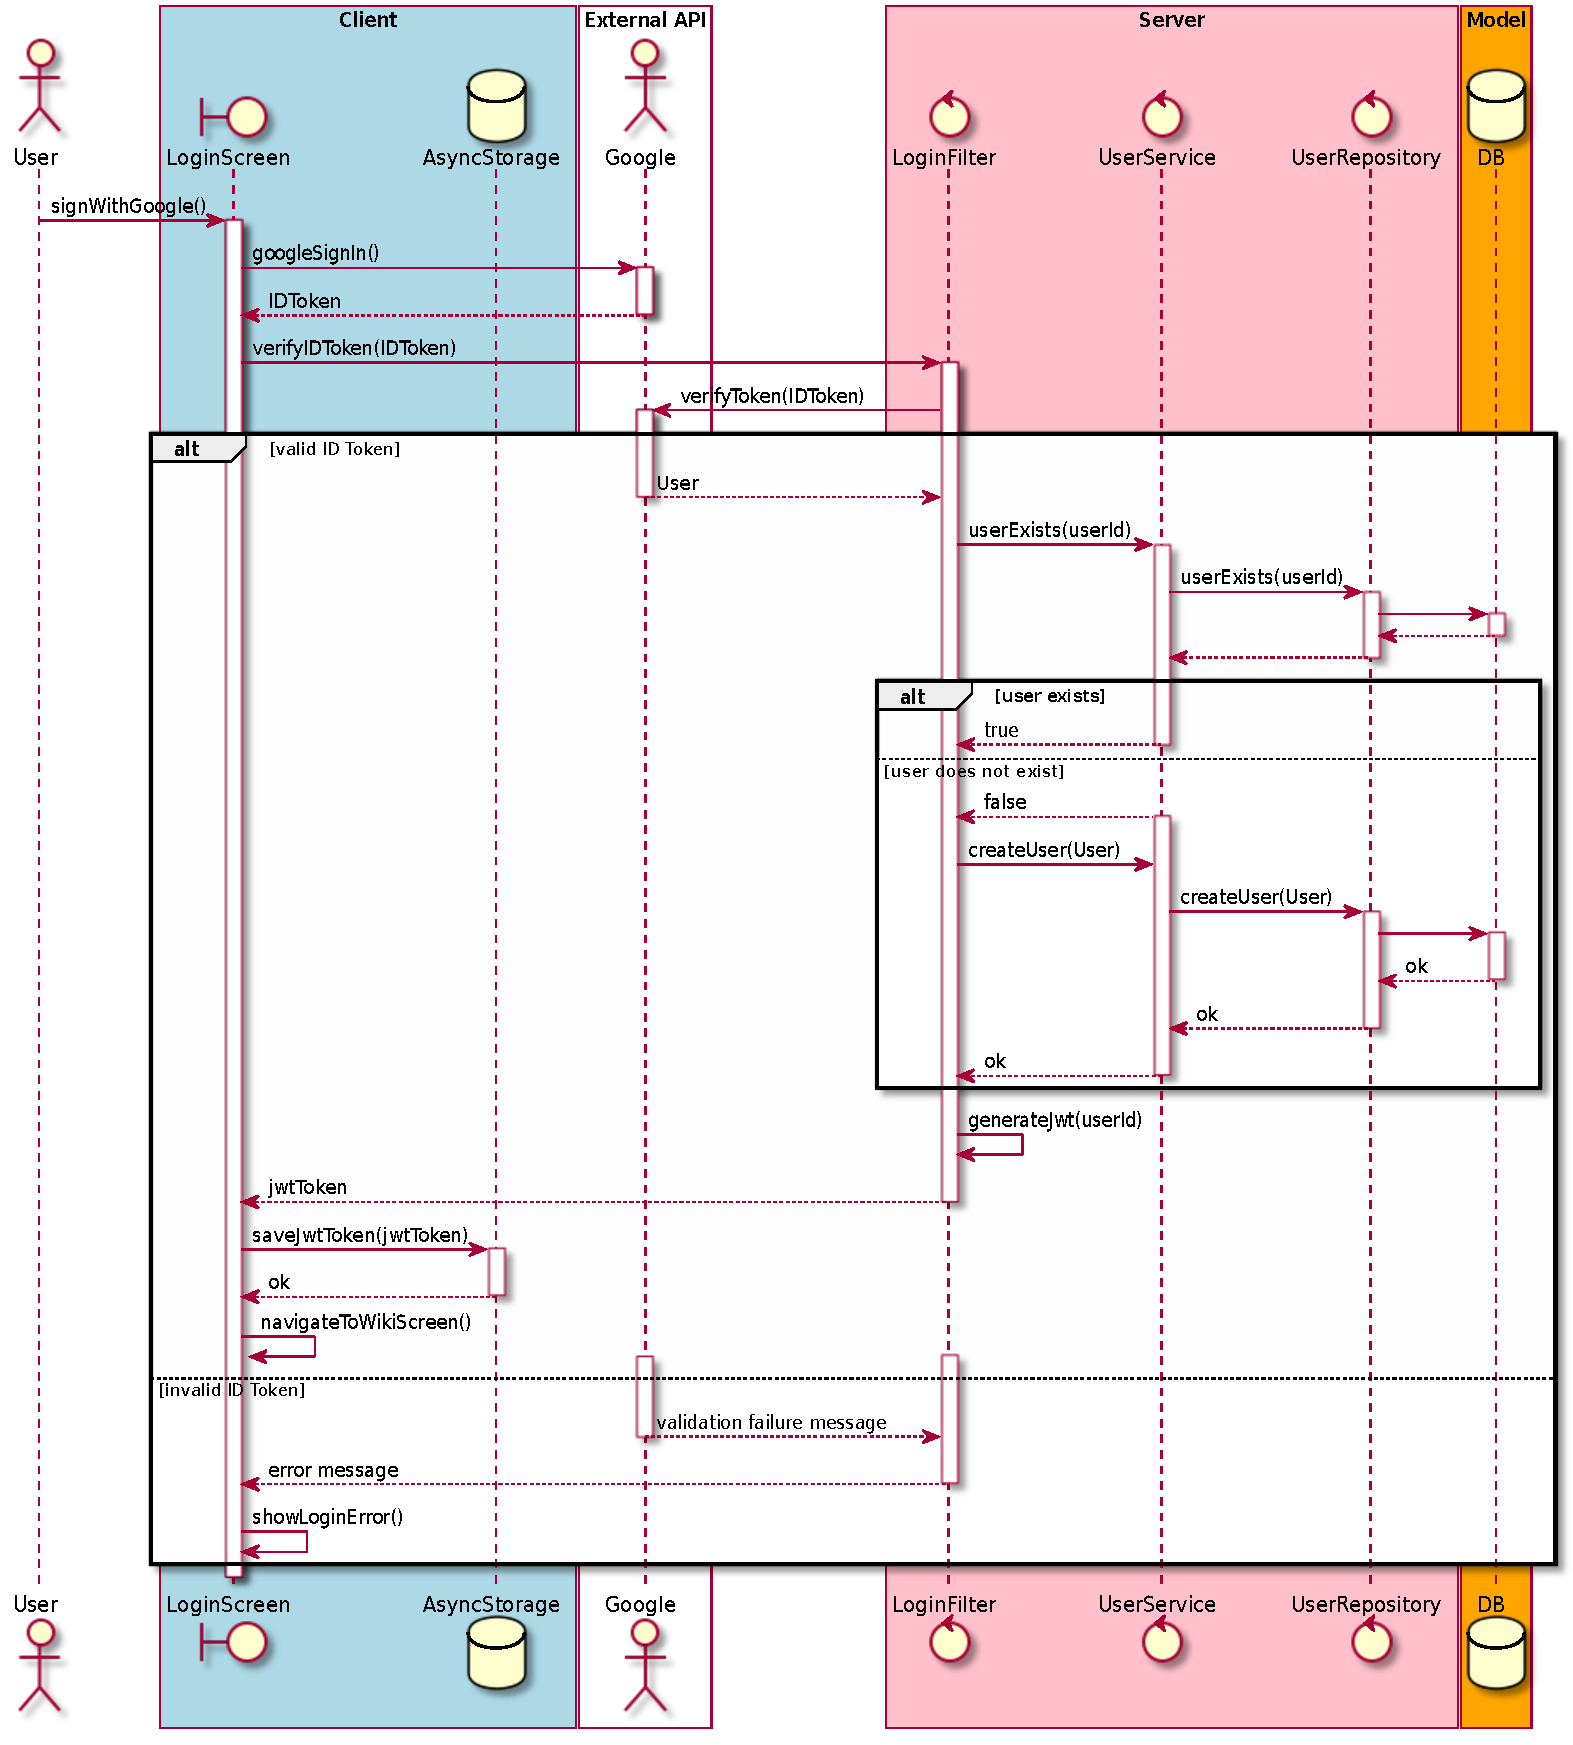
\includegraphics[width=\textwidth, keepaspectratio]{graphics/sequence_diagram_login.pdf}

\section{UC\_2 Dekoracja zapytania HTTP tokenem aktualnie zalogowanego użytkownika}
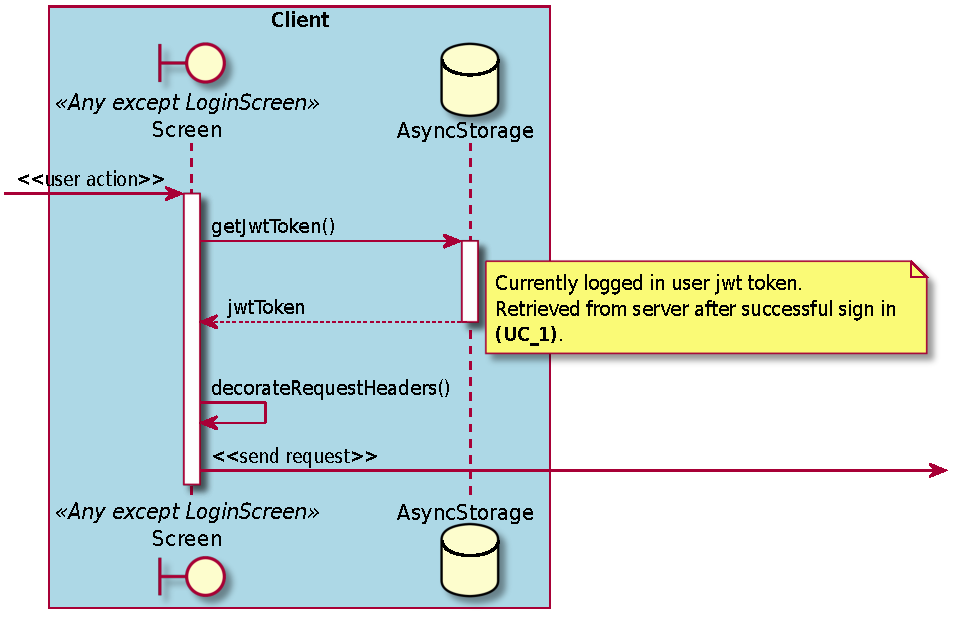
\includegraphics[width=\textwidth, keepaspectratio]{graphics/sequence_diagram_decorate_headers.pdf}

\section{UC\_3 Autentykacja użytkownika}
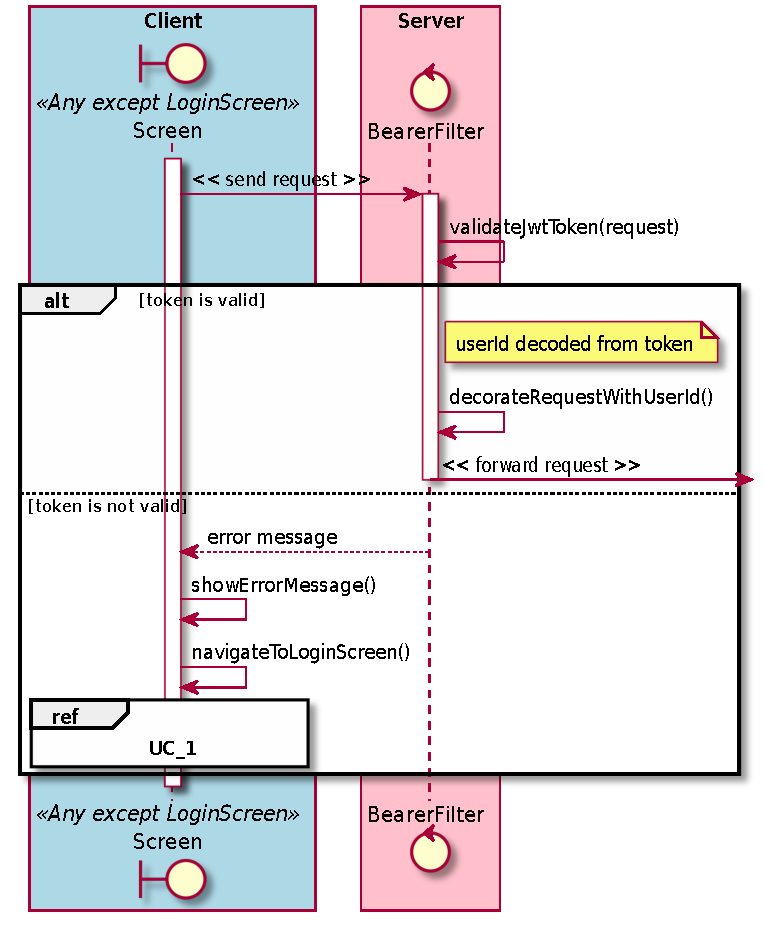
\includegraphics[width=\textwidth, keepaspectratio]{graphics/sequence_diagram_user_auth.pdf}

\section{UC\_4 Wyświetl listę wpisów w Wiki}
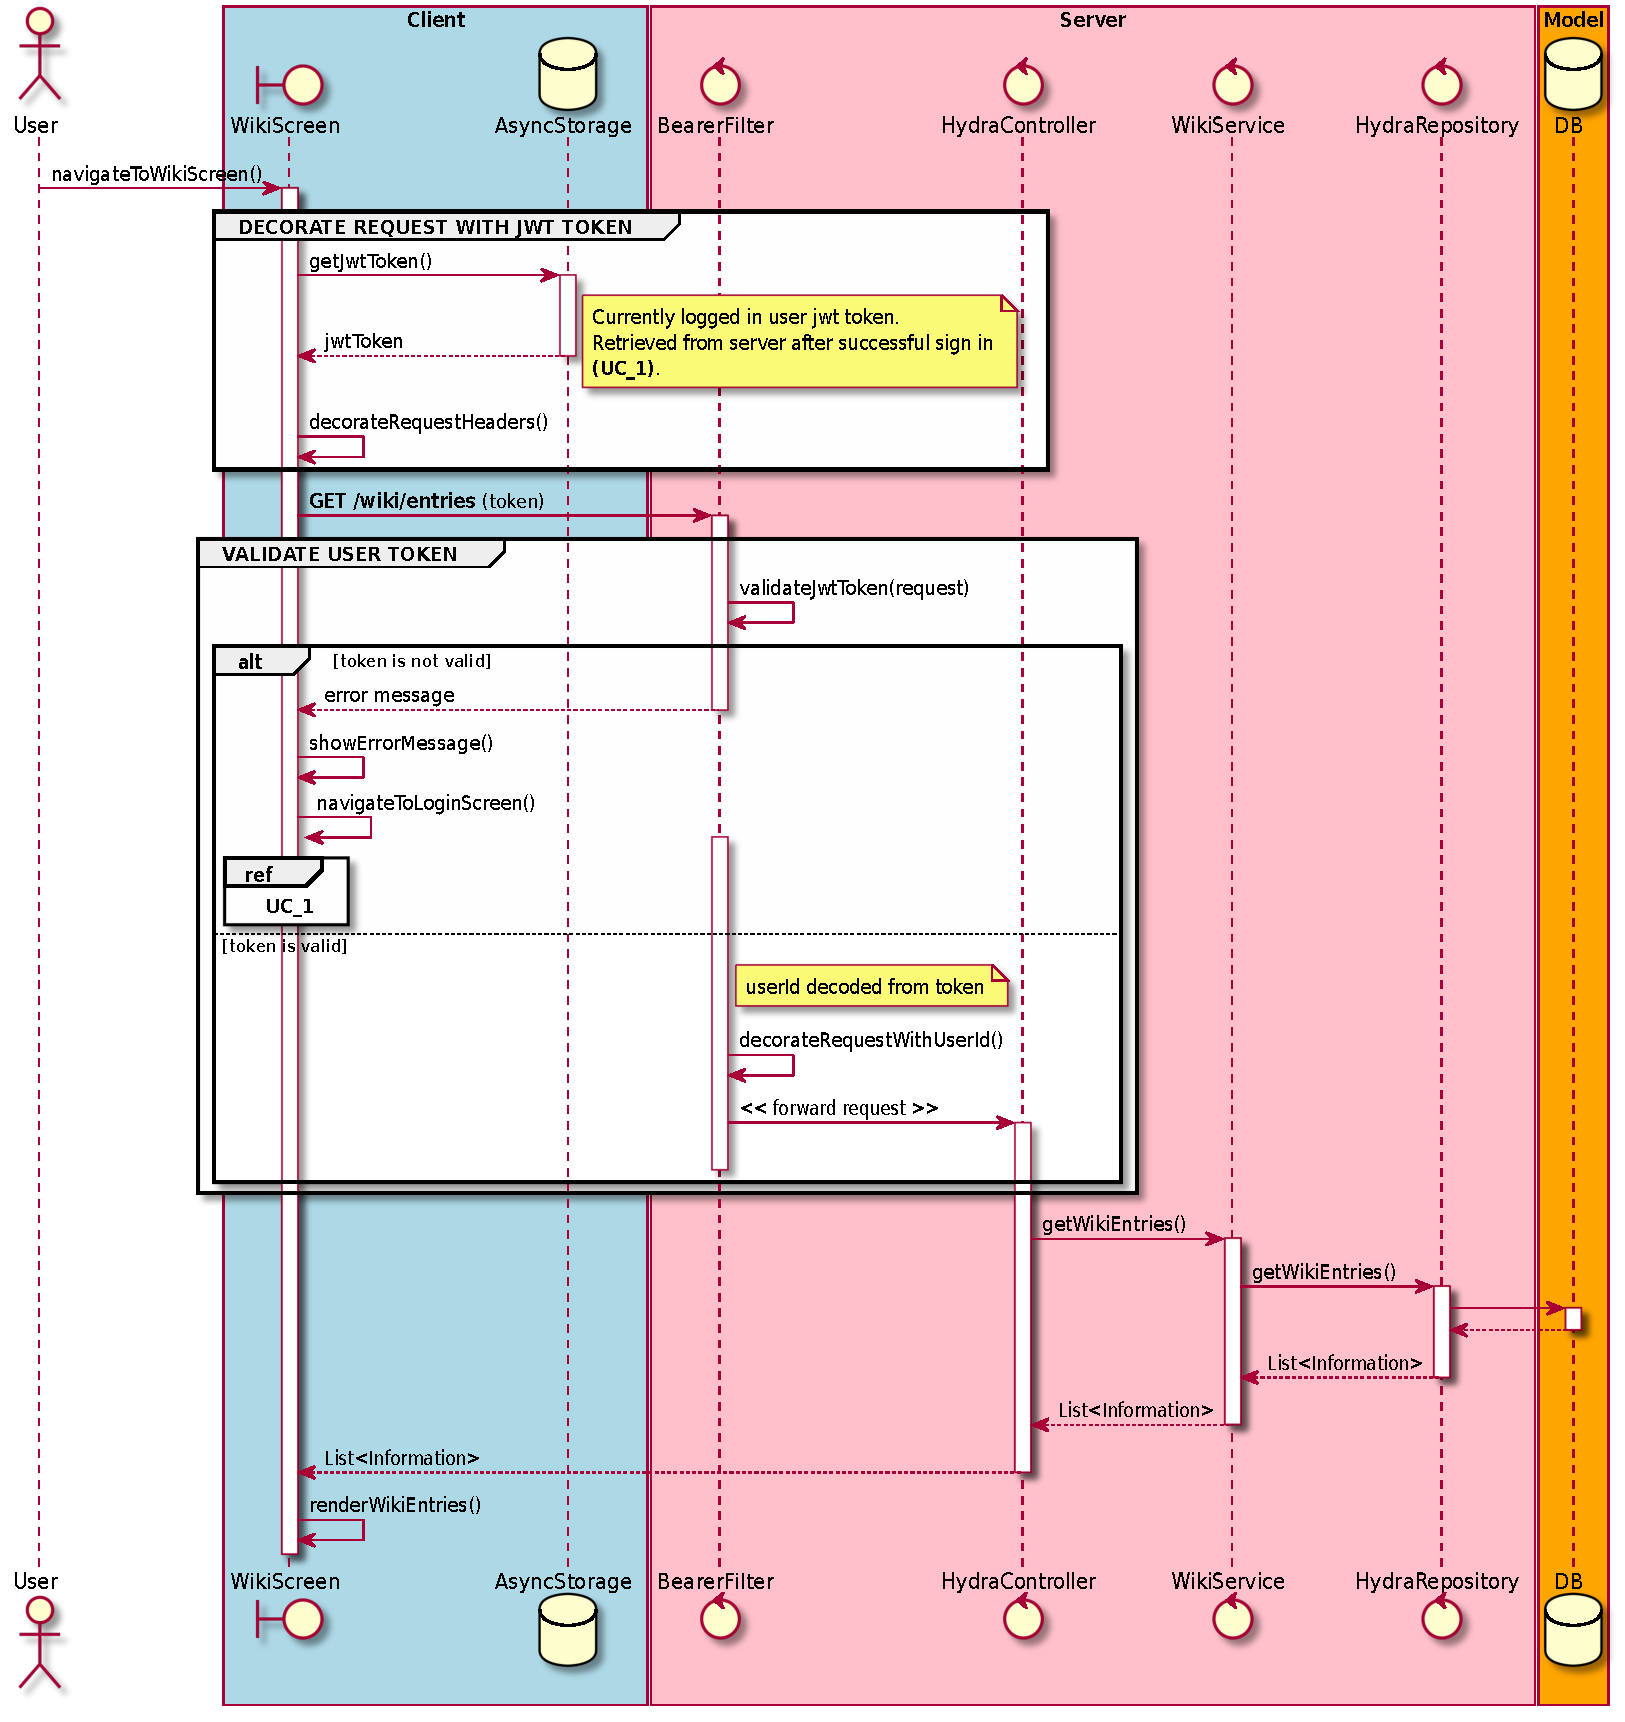
\includegraphics[width=\textwidth, keepaspectratio]{graphics/sequence_diagram_wiki_list.pdf}

\section{UC\_5 Dodaj wpis do Wiki}
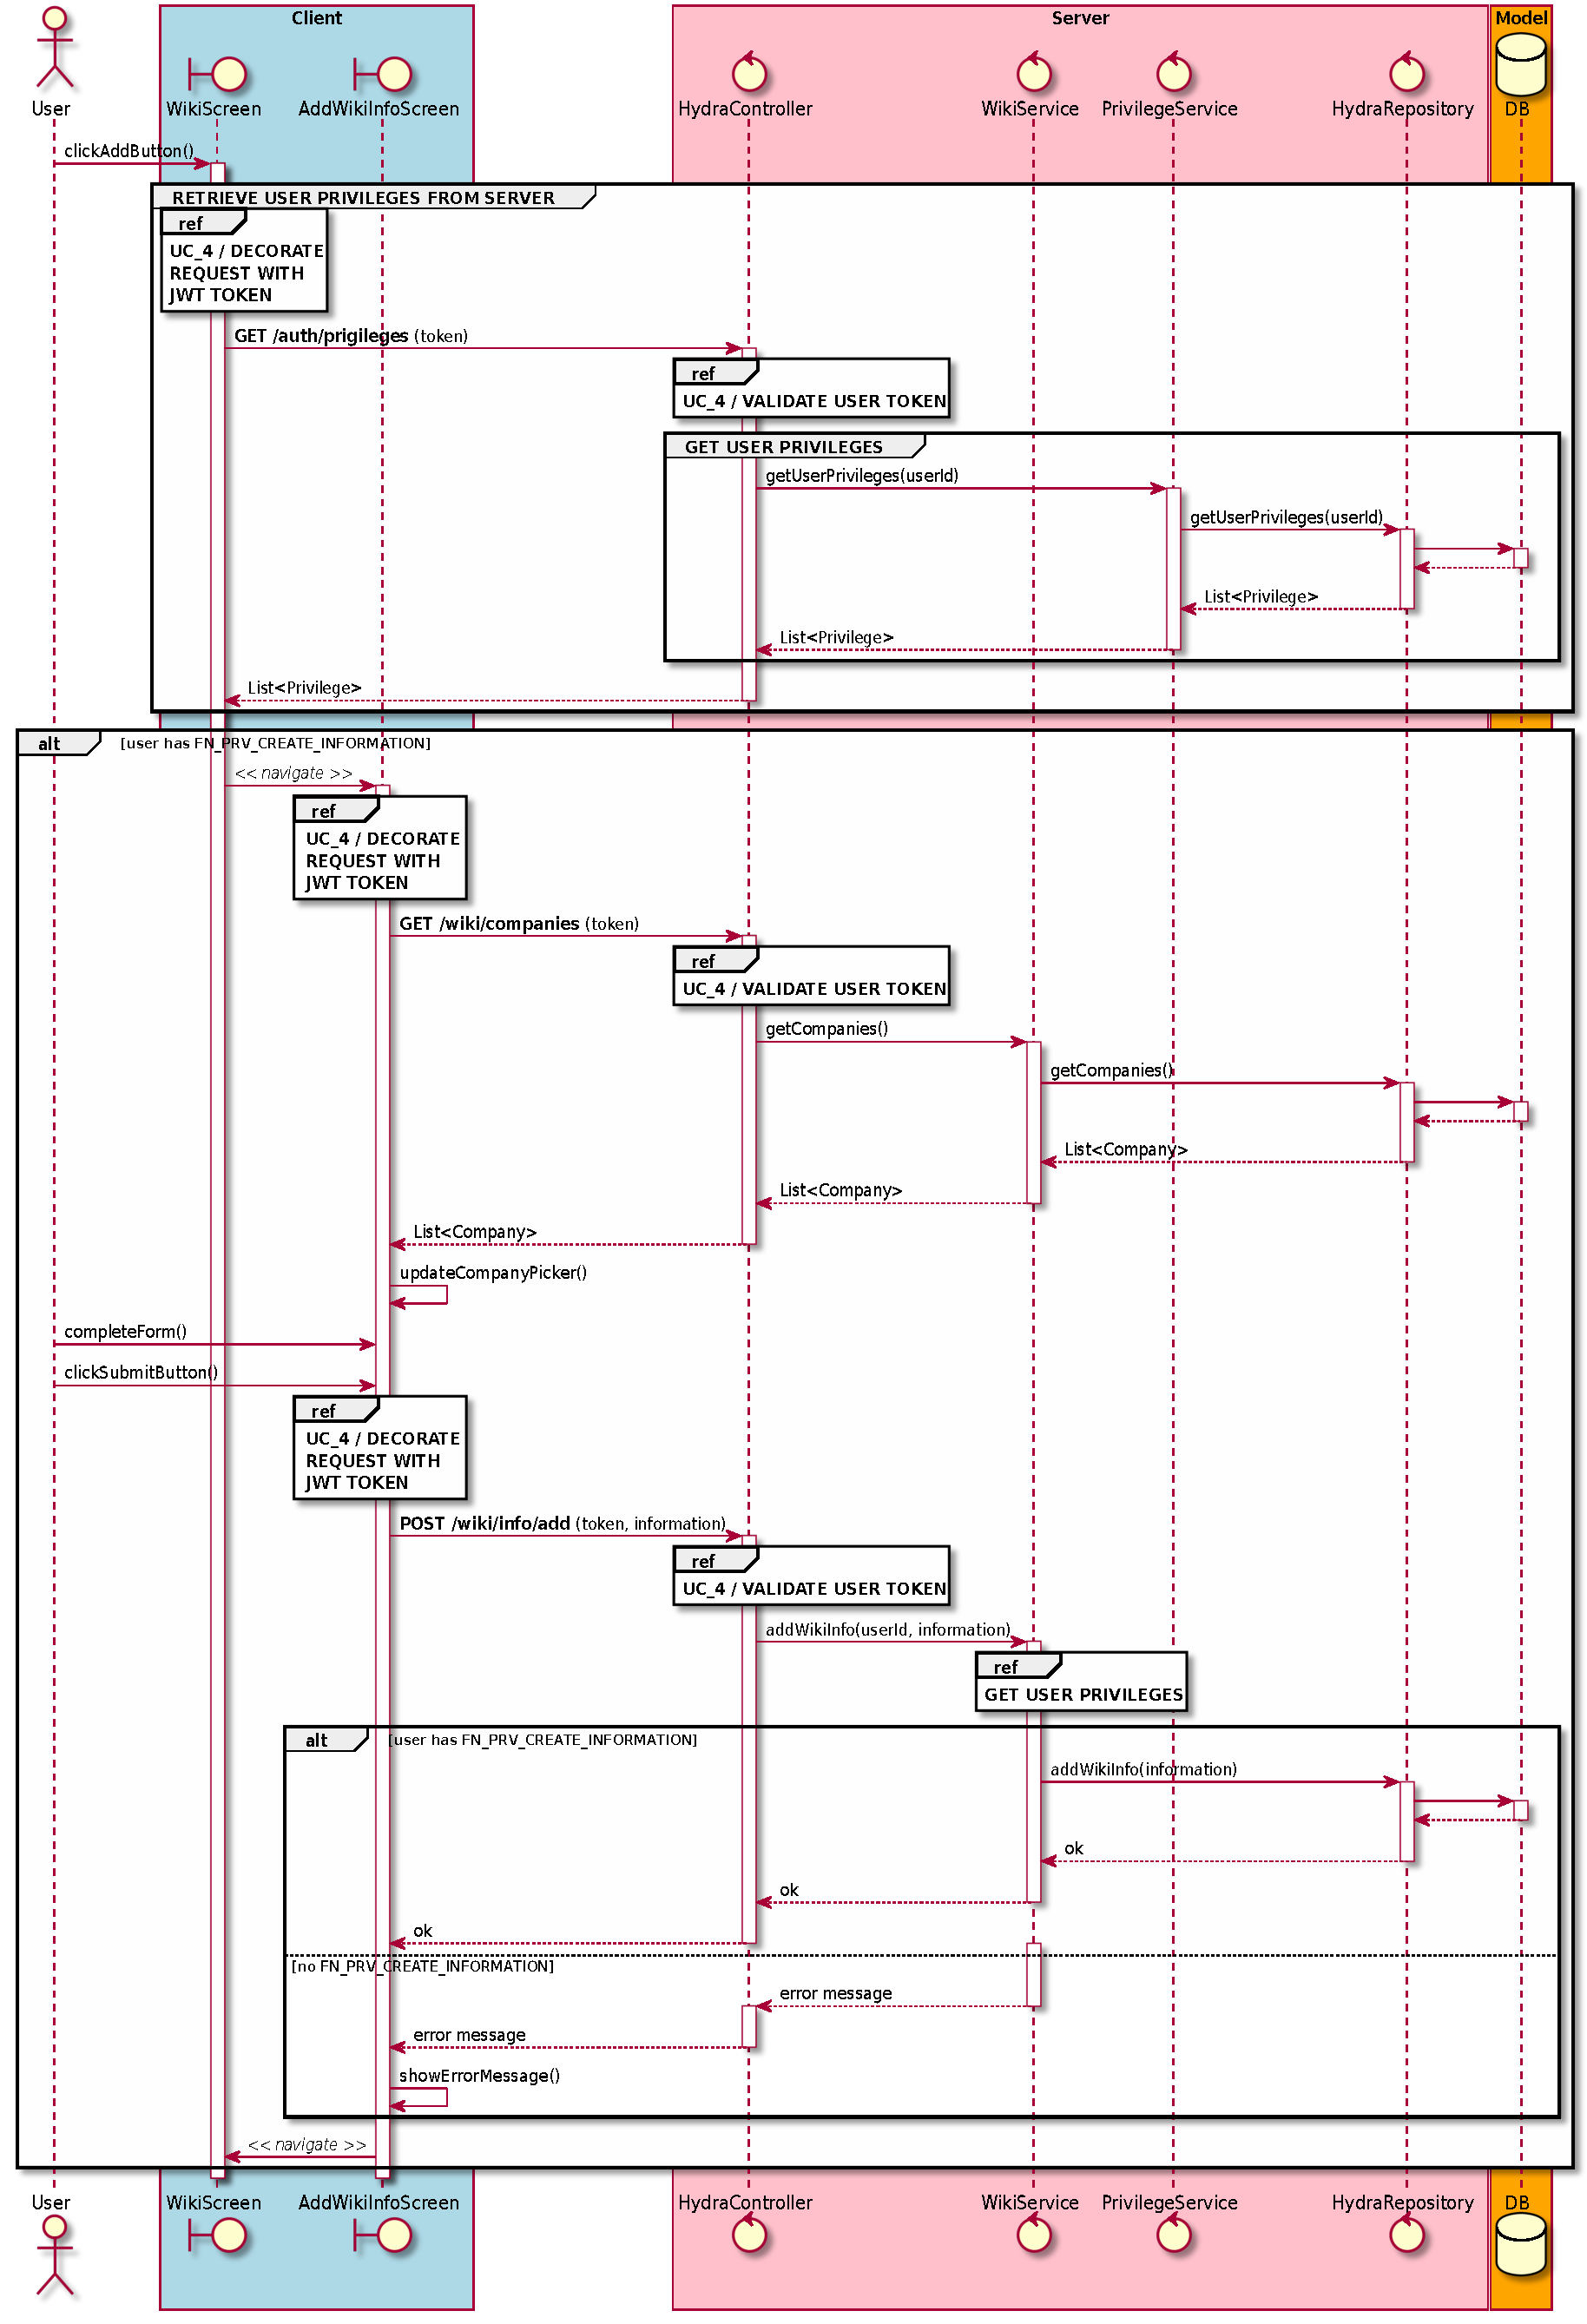
\includegraphics[width=\textwidth, keepaspectratio]{graphics/sequence_diagram_wiki_add.pdf}

\section{UC\_6 Zagłosuj na wpis na Wiki}
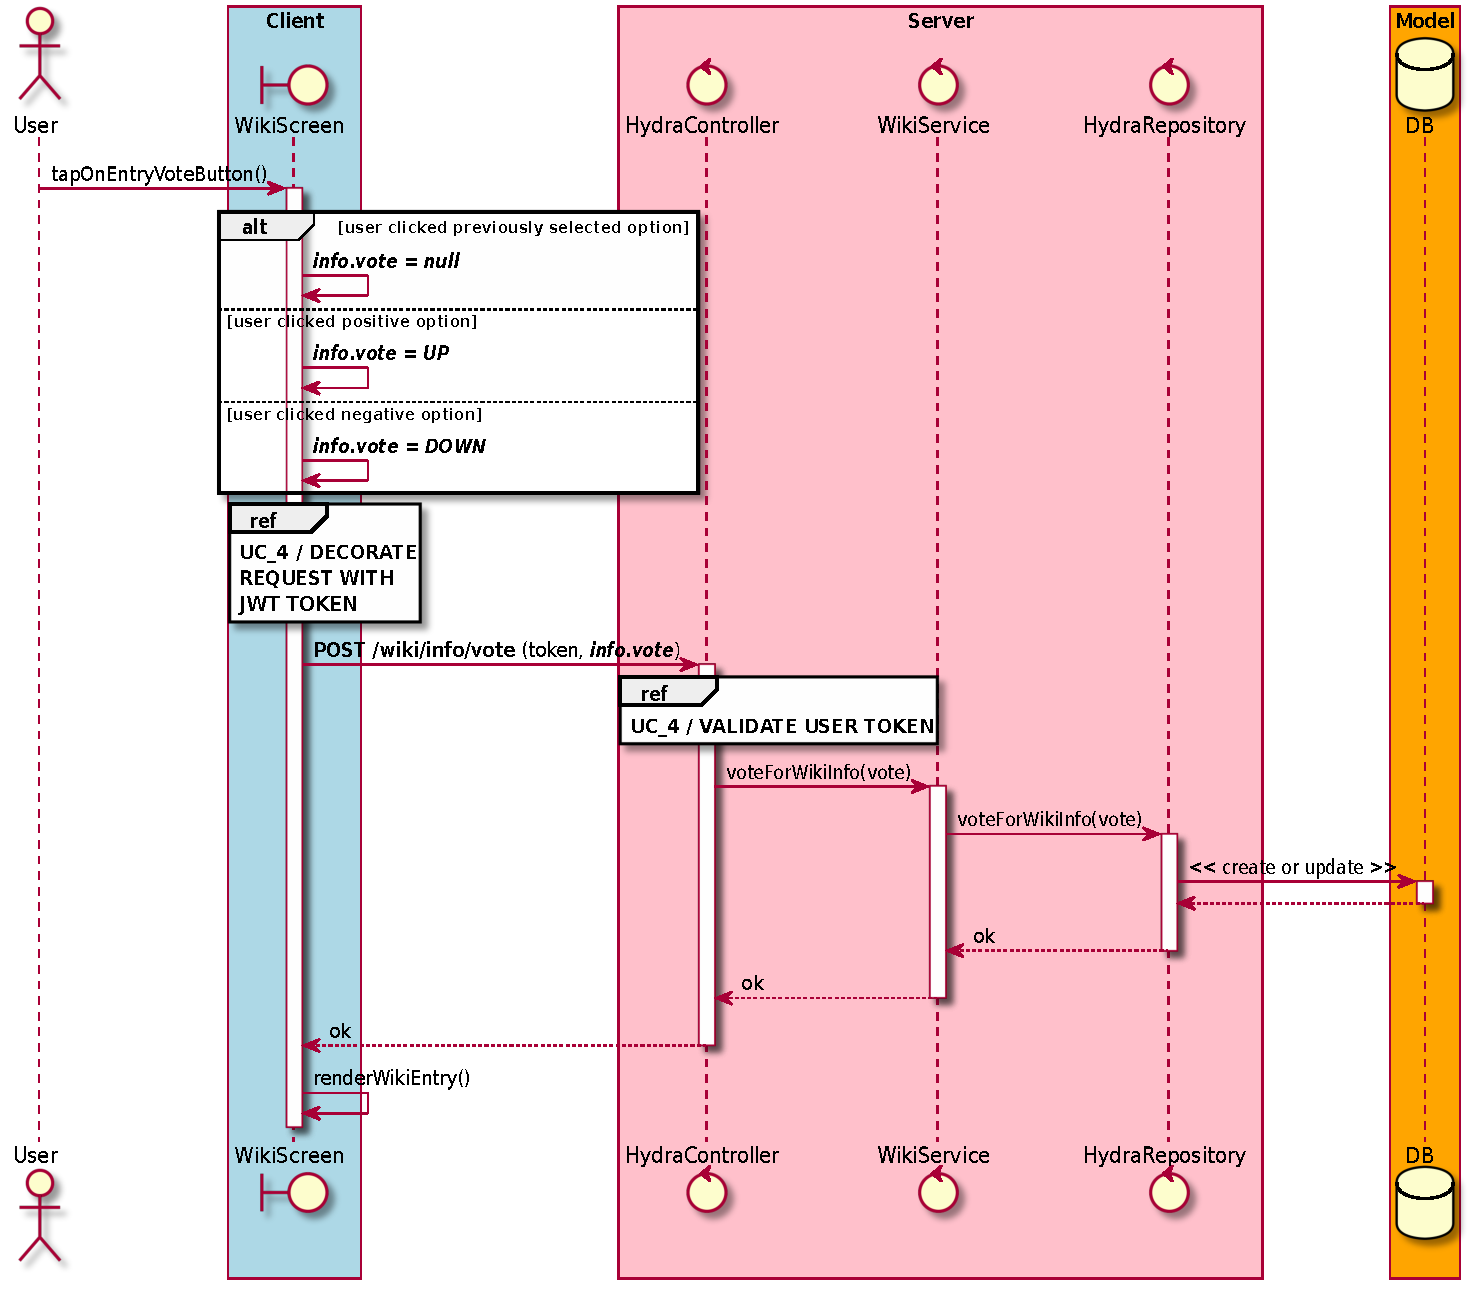
\includegraphics[width=\textwidth, keepaspectratio]{graphics/sequence_diagram_wiki_vote.pdf}

\section{UC\_7 Wyświetl listę ofert pracy}
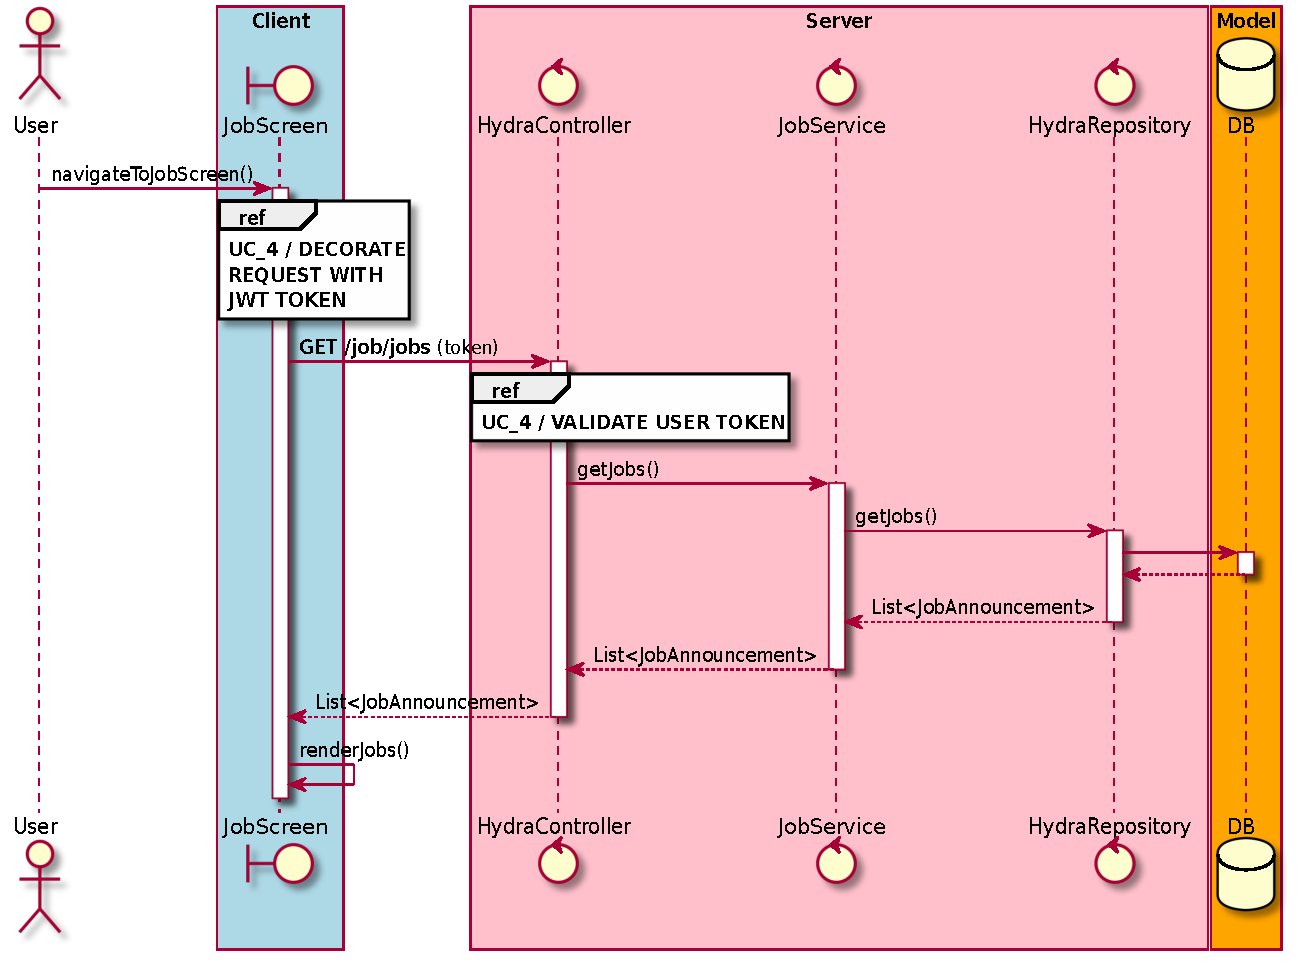
\includegraphics[width=\textwidth, keepaspectratio]{graphics/sequence_diagram_job_list.pdf}

\section{UC\_8 Wyświetl szczegóły oferty pracy}
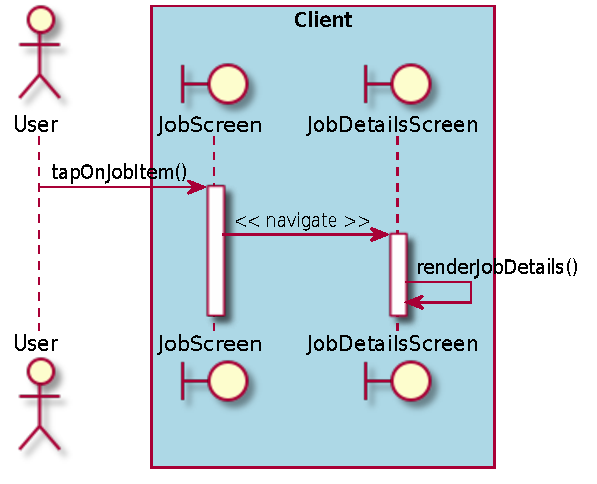
\includegraphics[width=\textwidth, keepaspectratio]{graphics/sequence_diagram_job_details.pdf}

\section{UC\_10 Wyświetl listę RA}
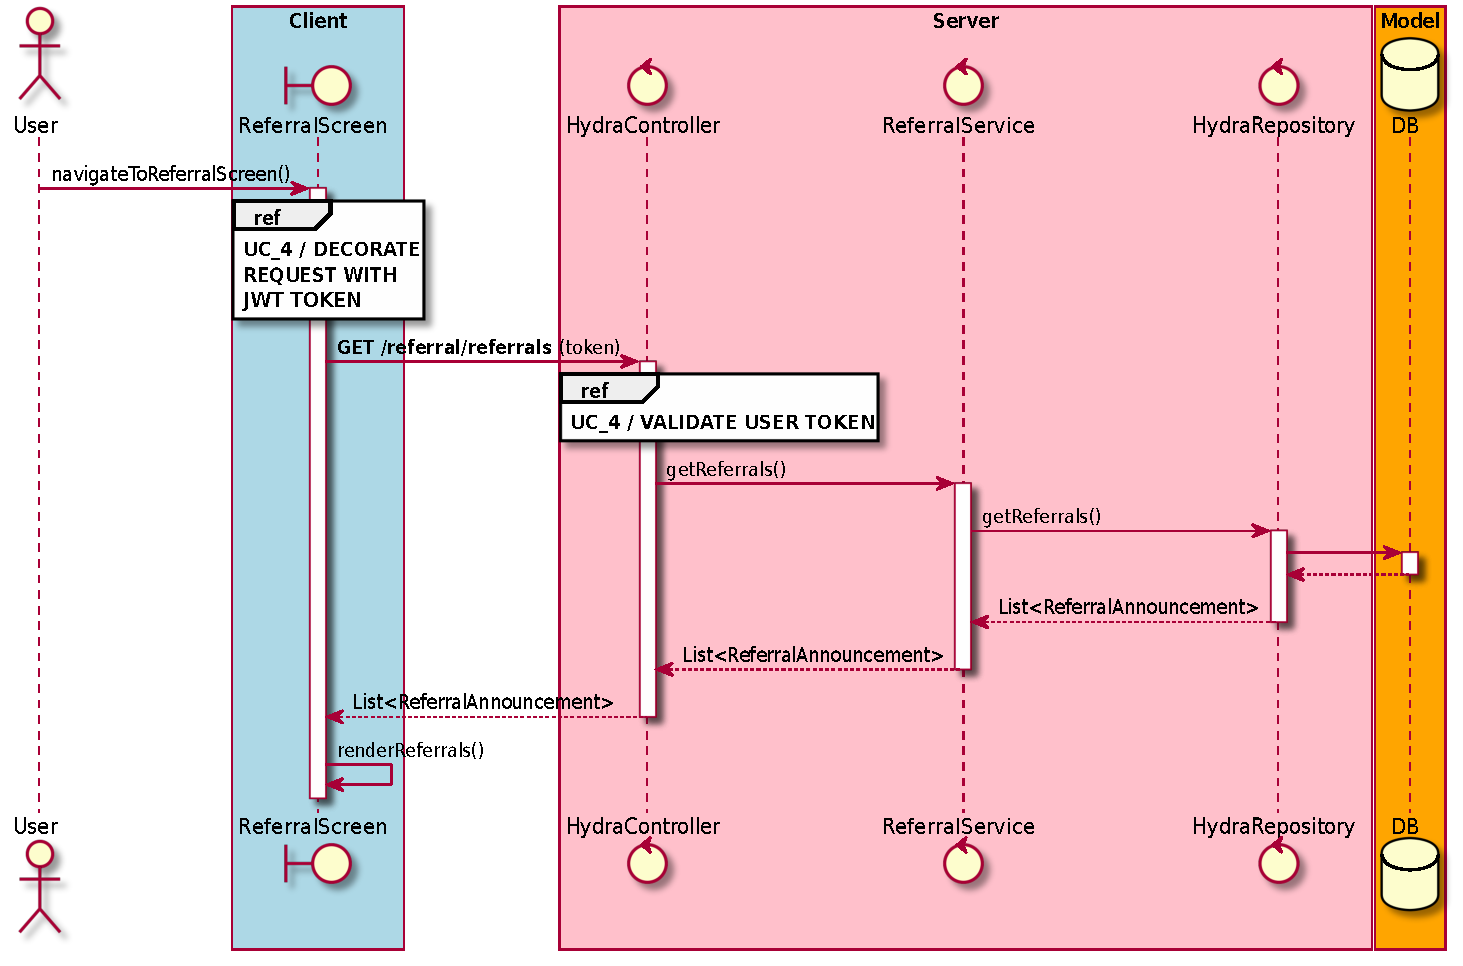
\includegraphics[width=\textwidth, keepaspectratio]{graphics/sequence_diagram_referral_list.pdf}


\chapter{Projekt interfejsu użytkownika IRS}

\section{Ekrany zorientowane wokół Wiki}
\begin{center}
	\makebox[\textwidth]{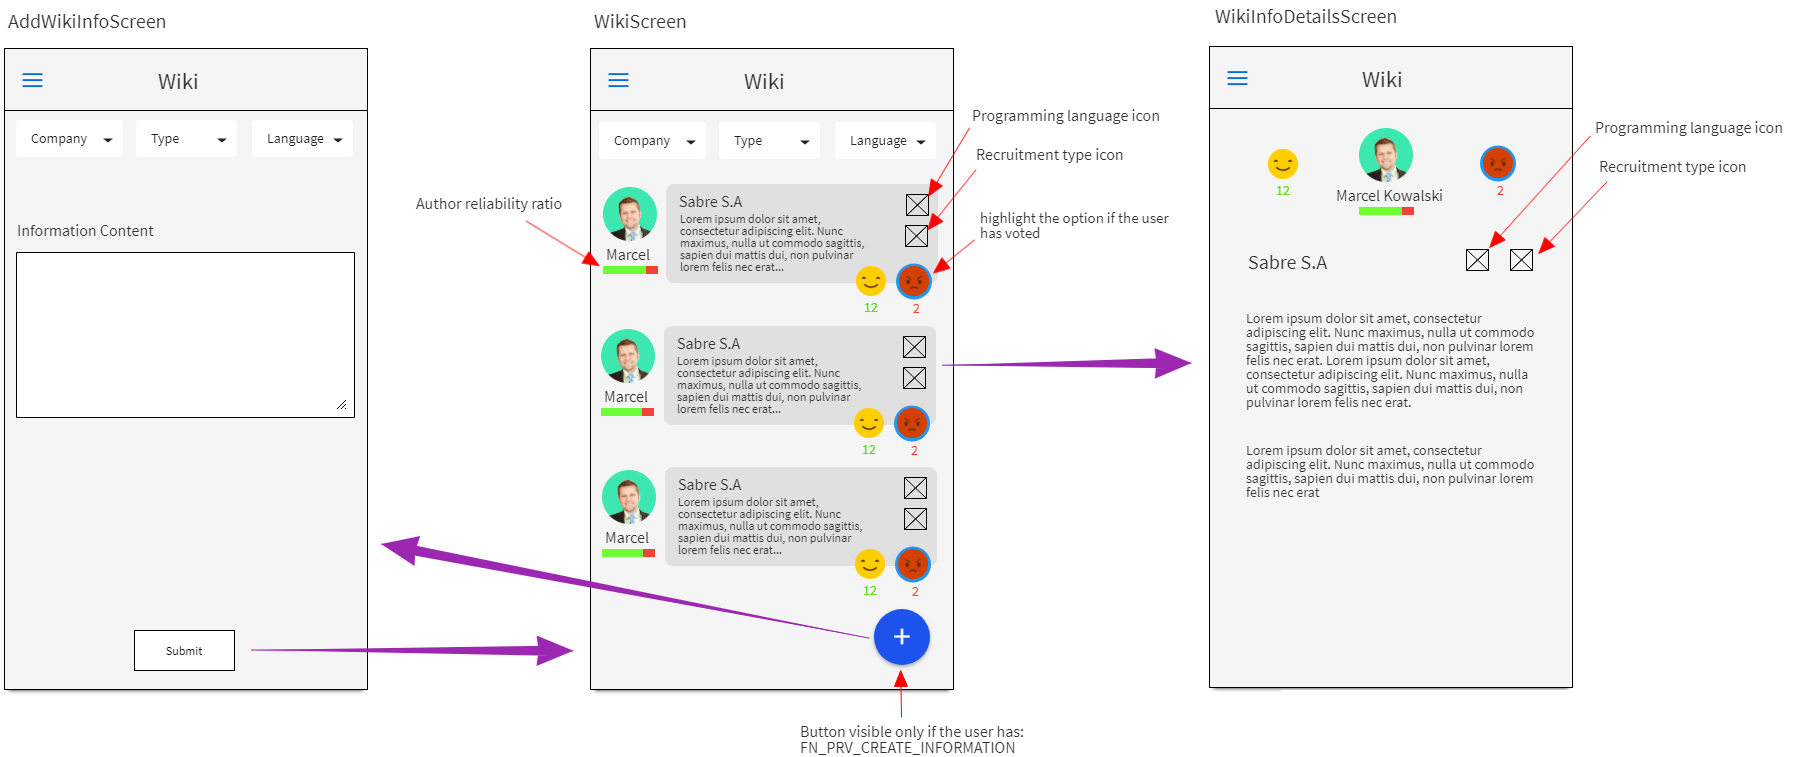
\includegraphics[width=\textwidth]{graphics/wiki_user_interface}}
\end{center}

\section{Ekrany zorientowane wokół Job i Referral}
\begin{center}
	\makebox[\textwidth]{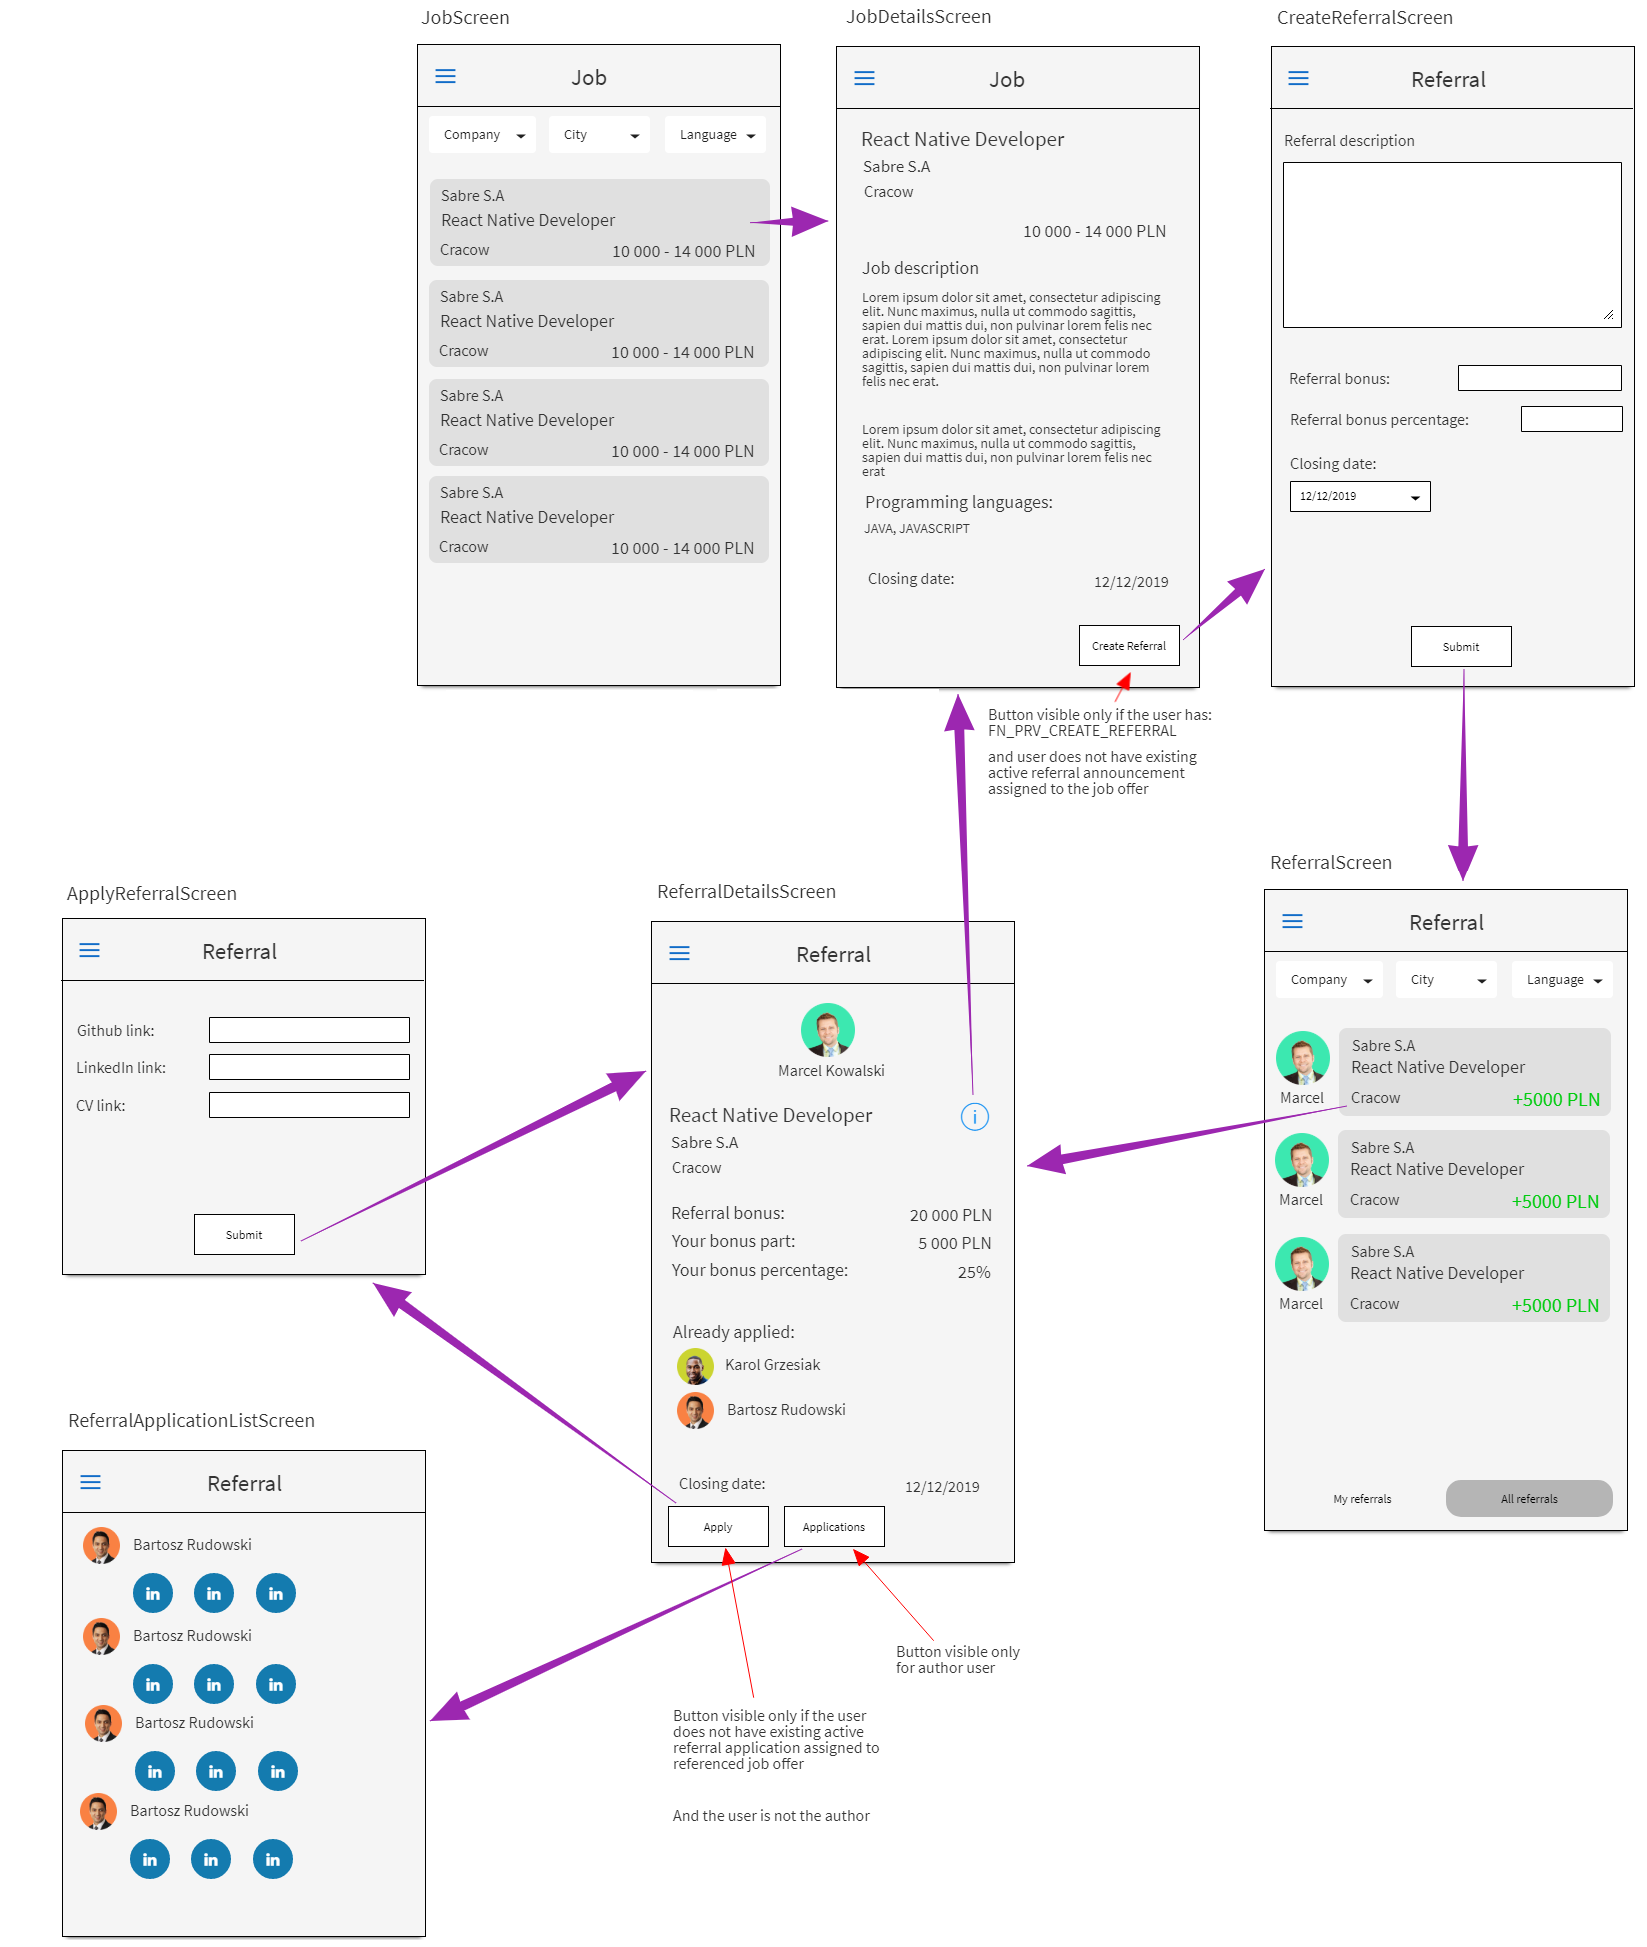
\includegraphics[width=\textwidth]{graphics/job_referral_user_interface}}
\end{center}


\chapter{Projekt bazy danych}

\section{Diagram ERD}
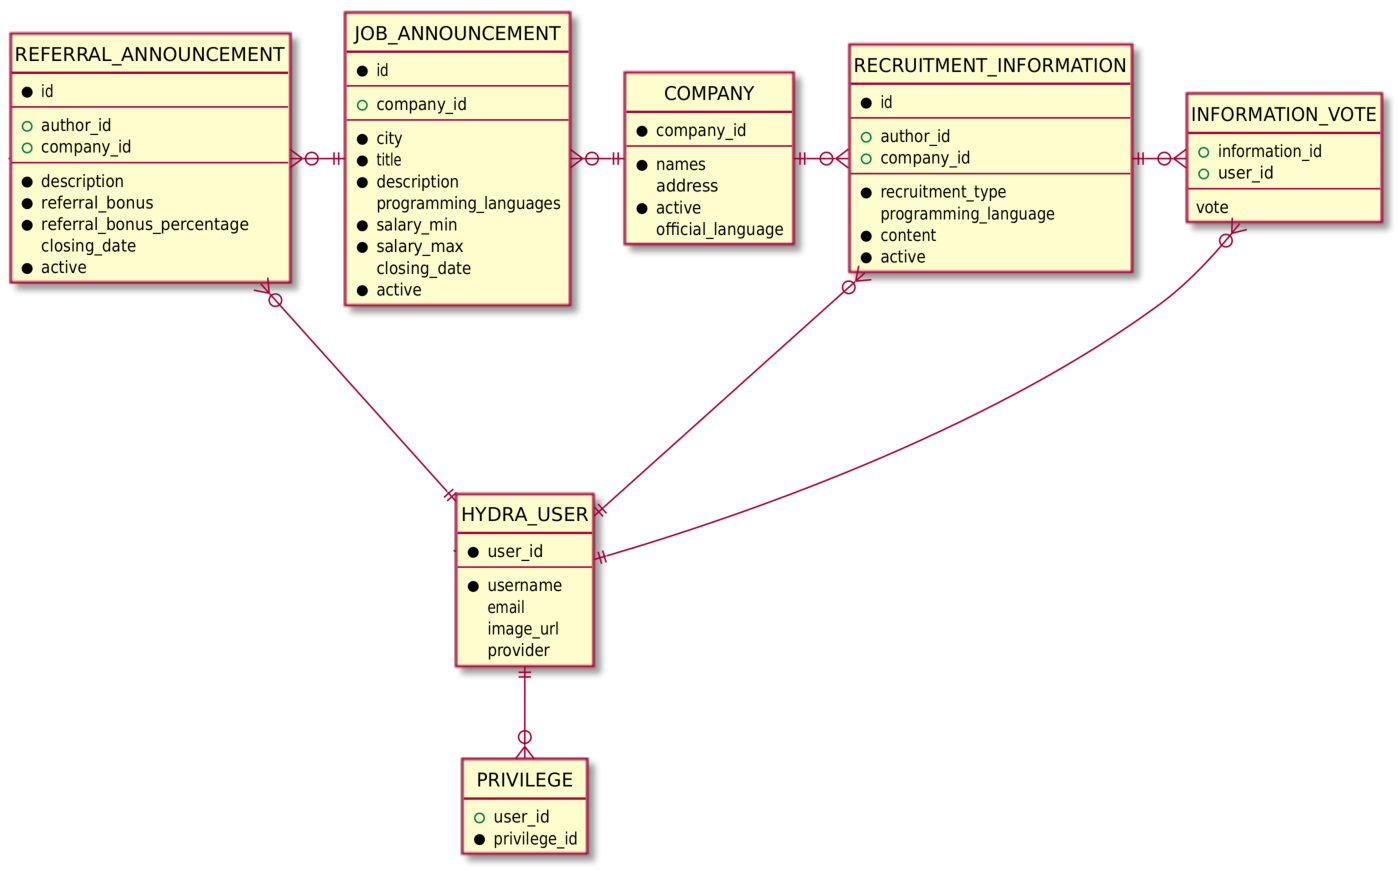
\includegraphics[width=\textwidth, keepaspectratio]{graphics/hydra_db_erd.pdf}

\section{Specyfikacja kwerend}
//TODO: Danon


\end{document}